\documentclass{article}

\usepackage[a4paper, total={6in, 8.5in}]{geometry}
\usepackage[utf8]{inputenc}
\usepackage[T1]{fontenc}    
\usepackage{hyperref} 
\usepackage{url}   
\usepackage{booktabs}    
\usepackage{amssymb,amsfonts,amsmath,graphicx}      
\usepackage{nicefrac}       
\usepackage{microtype}    
\usepackage{breqn}
\usepackage[usenames, dvipsnames]{color}

\newcommand{\ind}[1]{1_{#1}} % Indicator function
\newcommand{\pr}{P} % Generic probability
\newcommand{\ex}{E} % Generic expectation
\newcommand{\var}{\textrm{Var}}
\newcommand{\cov}{\textrm{Cov}}
\newcommand{\sgn}{\textrm{sgn}}
\newcommand{\sign}{\textrm{sign}}
\newcommand{\kl}{\textrm{KL}} 
\newcommand{\abs}[1]{|{#1}|}



\renewcommand{\S}{\Sigma}
\renewcommand{\L}{\Lambda}
\renewcommand{\[}{\begin{equation}}
\renewcommand{\]}{\end{equation}}
\renewcommand{\b}{\backslash}
\newcommand{\g}{\,\vert\,}
\newcommand{\tr}{\mathrm{tr}}
\newcommand{\diag}{\mathrm{diag}}
\newcommand{\bea}{\begin{eqnarray}}
\newcommand{\eea}{\end{eqnarray}}
\newcommand{\hx}{\hat{x}}
\newcommand{\hxi}{\hat{\xi}}
\newcommand{\Var}{\mathrm{Var}}
\newcommand{\Cov}{\mathrm{Cov}}
\newcommand{\prop}{\propto}
\newcommand{\deq}{:=}

\newcommand{\EE}{\mathbb{E}}
\newcommand{\II}{\mathbb{I}}
\newcommand{\R}{\mathbb{R}}
\newcommand{\PP}{\mathbb{P}}

\newcommand{\La}{\mathcal{L}}

\newcommand{\n}{\mathcal{N}}

\newcommand{\bx}{\mathbf{x}}
\newcommand{\bX}{\mathbf{X}}
\newcommand{\by}{\mathbf{y}}
\newcommand{\bs}{\mathbf{s}}
\newcommand{\bn}{\mathbf{n}}
\newcommand{\br}{\mathbf{r}}
\newcommand{\bt}{\mathbf{t}}

\newcommand{\fig}[1]{Figure~\ref{fig:#1}}
\newcommand{\chap}[1]{Chapter~\ref{chap:#1}}
\newcommand{\mysec}[1]{Section~\ref{sec:#1}}
\newcommand{\app}[1]{Appendix~\ref{sec:#1}}
\newcommand{\eq}[1]{Eq.~(\ref{eq:#1})}
\newcommand{\eqs}[1]{Eqs.~(\ref{eq:#1})}
\newcommand{\eqss}[1]{(\ref{eq:#1})}
\newcommand{\thm}[1]{Theorem~\ref{thm:#1}}

\newcommand{\indep}{{\;\bot\!\!\!\!\!\!\bot\;}}
\newcommand{\eps}{\varepsilon}

\newcommand{\one}{1}
\newcommand{\Dir}{{\rm Dir}}
\newcommand{\Mult}{{\rm Mult}}
\newcommand{\Bin}{{\rm Bin}}
\newcommand{\Ga}{{\rm Ga}}
\newcommand{\IG}{{\rm IG}}
\newcommand{\InvGa}{{\rm IG}}
\newcommand{\Chisquare}{\Chi^2}
\newcommand{\St}{{\rm St}}
\newcommand{\Beta}{{\rm Beta}}
\newcommand{\iid}{i.i.d.}
\newcommand{\Eta}{{\cal N}}
\newcommand{\Ber}{{\rm Ber}}

\newcommand{\simiid}{\stackrel{\tiny\text{iid}}{\sim}}
\newcommand{\simind}{\stackrel{\tiny\text{ind}}{\sim}}

\DeclareMathOperator*{\BP}{BP}
\DeclareMathOperator*{\DP}{DP}
\DeclareMathOperator*{\GP}{GP}
\DeclareMathOperator*{\BeP}{BeP}

% Caligraphic alphabet
\newcommand{\calr}{\mathcal{R}} % only because \cr already taken
\newcommand{\ca}{\mathcal{A}} \newcommand{\cb}{\mathcal{B}} \newcommand{\cc}{\mathcal{C}} \newcommand{\cd}{\mathcal{D}} \newcommand{\ce}{\mathcal{E}} \newcommand{\cf}{\mathcal{F}} \newcommand{\cg}{\mathcal{G}} \newcommand{\ch}{\mathcal{H}} \newcommand{\ci}{\mathcal{I}} \newcommand{\cj}{\mathcal{J}} \newcommand{\ck}{\mathcal{K}} \newcommand{\cl}{\mathcal{L}} \newcommand{\cm}{\mathcal{M}} \newcommand{\cn}{\mathcal{N}} \newcommand{\co}{\mathcal{O}} \newcommand{\cp}{\mathcal{P}} \newcommand{\cq}{\mathcal{Q}} \newcommand{\cs}{\mathcal{S}} \newcommand{\ct}{\mathcal{T}} \newcommand{\cu}{\mathcal{U}} \newcommand{\cv}{\mathcal{V}} \newcommand{\cw}{\mathcal{W}} \newcommand{\cx}{\mathcal{X}} \newcommand{\cy}{\mathcal{Y}} \newcommand{\cz}{\mathcal{Z}}

% Convergence
\newcommand{\convd}{\stackrel{d}{\longrightarrow}} % convergence in distribution/law/measure
\newcommand{\convp}{\stackrel{P}{\longrightarrow}} % convergence in probability
\newcommand{\convas}{\stackrel{\textrm{a.s.}}{\longrightarrow}} % convergence almost surely
\newcommand{\convr}{\stackrel{r}{\longrightarrow}} % convergence in r^{th} mean

\newcommand{\eqd}{\stackrel{d}{=}} % equal in distribution/law/measure
\newcommand{\argmax}{\mathop{\mathrm{argmax}}}
\newcommand{\argmin}{\mathop{\mathrm{argmin}}}
\newcommand{\conv}{\textrm{conv}} % for denoting the convex hull


\makeatletter
\providecommand*{\diff}%
	{\@ifnextchar^{\DIfF}{\DIfF^{}}}
\def\DIfF^#1{%
	\mathop{\mathrm{\mathstrut d}}%
		\nolimits^{#1}\gobblespace}
\def\gobblespace{%
	\futurelet\diffarg\opspace}
\def\opspace{%
	\let\DiffSpace\!%
	\ifx\diffarg(%
		\let\DiffSpace\relax
	\else
		\ifx\diffarg[%
			\let\DiffSpace\relax
	\else
		\ifx\diffarg\{%
			\let\DiffSpace\relax
		\fi\fi\fi\DiffSpace}


\providecommand*{\deriv}[3][]{\frac{\diff^{#1}#2}{\diff #3^{#1}}}
\providecommand*{\pderiv}[3][]{\frac{\partial^{#1}#2}{\partial #3^{#1}}}
		
\newcommand{\threequals}{\equiv}

\DeclareMathOperator*{\argminU}{arg\,min}
\DeclareMathOperator*{\argmaxU}{arg\,max}


\begin{document}


\section{Model}
\label{model}


\noindent Stochastic Block Model (SBM)
\begin{itemize}
\item Choose the community proportions $\pi \sim \text{Dir}(\gamma)$, where $\pi\in \R^C$ with $C$ latent communities
\item For each representative $u$
\begin{enumerate}
\item Choose a community membership assignment $M_u\simiid \text{Cat}(\pi)$
\end{enumerate}
\item For each pair of communities $k, l\in\{1,\dots, C\}$, draw coexpression rate $P_{kl} \simiid \text{Gamma}(\lambda_0,\lambda_1)$%, for $k,l\in \{1,\dots, C\}$
\item For each pair of representatives $u,v\in\{1,\dots, U\}$, draw $R_{uv} \mid P, M_u=k, M_v=l\sim \text{Poisson}(P_{kl})$
\end{itemize}


\noindent Ideal Point Model (IPM)
\begin{itemize}
\item For each document $d$
\begin{enumerate}
\item Choose a discrimination $a_d \sim \cn(\eta_{a},\sigma^2_d)$
\item Choose a difficulty $b_d \sim \cn(\eta_{b},\sigma^2_d)$
\end{enumerate}
\item For each representative $u$
\begin{enumerate}
\item Choose a position $x_u\mid \nu \sim \cn(\nu,\sigma^2_x)$
\end{enumerate}
\item Draw representative $u$'s vote on document $d$ as $V_{ud} \mid x_u, a_d, b_d \sim \text{Bern}(\sigma(a_d\cdot(x_u-b_d)))$%, for $u\in\{1,\dots, U\}, d\in\{1,\dots,D\}$
\end{itemize}

\noindent Latent Dirichlet Allocation (LDA)
\begin{itemize}
\item Draw a topic $\varphi_k \simiid \text{Dir}(\beta), \varphi_k\in \R^V$ as a distribution over words, for each $k\in\{1,\dots,K\}$ 
\item For each document, draw the topic proportions $\theta_d \simiid \text{Dir}(\alpha)$, where $\theta_d\in \R^K$ %, for $d\in\{1,\dots,D\}$
\item For each document $d\in\{1,\dots,D\}$ and each word $n\in\{1,\dots,N_d\}$ in the document
\begin{enumerate}
\item Choose a topic $z_{dn}\mid \theta_d \simind \text{Mult}(\theta_d)$ %, for $d\in\{1,\dots,D\}$, $n\in\{1,\dots,N_d\}$
\item Choose a word $W_{dn}\mid z_{dn}=k, \varphi_k\simind \text{Mult}(\varphi_k)$ %, for $d\in\{1,\dots,D\}$, $n\in\{1,\dots,N_d\}$
\end{enumerate}
\end{itemize}


\newpage


\subsection{Frankenstein Model}

The ideal point model (IPM) is useful to us as a baseline model for the roll call voting data $(V_{ud})$ for a couple of reasons. For one, using it alone we can attempt to predict missing votes, a problem of interest in political science. Another problem of more qualitative interest is analyzing and interpreting the factors $a_d, b_d$ specific to a document and those $x_u$ specific to the representative. All are assumed to reside in some latent space $\R^S$ and so depending on how we set up the model, we might be able to interpret quantities like $x_u$ as $u$'s {\sl political stance} or {\sl ideological position} or $x_u - b_d$ as representative $u$'s propensity for the bill/document $d$. There are a number of problems we cannot address in IPM. A major problem is predicting on heldout documents (the `cold start'), which is a potentially useful performance measure. Similarly if we have relatively junior representatives, they may not have had enough votes for the inferred $x_u$ to represent something (1) meaningful / interpretable or (2) reliable. We want to incorporate more information to inform the choices of $a_d, b_d$ and $x_u$. \\


\noindent Ideal Point Allocator (IPA)
\begin{itemize}
\item Run the generative processes for SBM and LDA as described above. Then,
\item For each document $d$
\begin{enumerate}
\item Calculate the empirical topic proportions $\overline z_d  = \frac{1}{N_d}\sum_{i=1}^{N_d}z_d$ (a $K\times 1$ vector)
\item Generate $S\times K$ matrices $\eta_a, \eta_b$ with iid normal entries 
\item Choose a discrimination $a_d \sim \cn(\eta_{a}'\overline z_d,\sigma^2_d)$
\item Choose a difficulty $b_d \sim \cn(\eta_{b}'\overline z_d,\sigma^2_d)$
\end{enumerate}
\item For each representative $u$
\begin{enumerate}
\item Generate the community means $\nu_k\sim \cn(\tau, \sigma^2_x)$
\item Choose a position $x_u\mid M_u = k, \nu \sim \cn(\nu_k,\sigma^2_x)$
\end{enumerate}
\item Draw representative $u$'s vote on document $d$ as $V_{ud} \mid x_u, a_d, b_d \sim \text{Bern}(\sigma(a_d\cdot(x_u-b_d)))$
\end{itemize}



\begin{figure}[h]
  \centering
  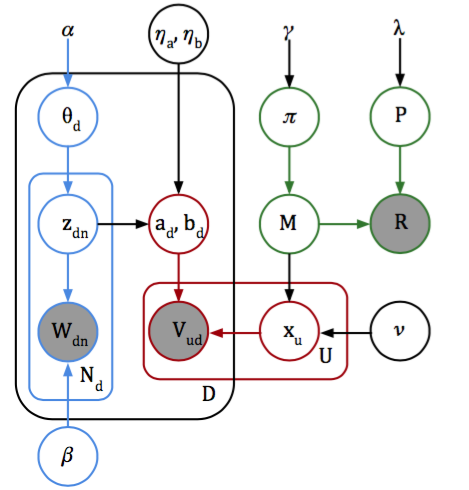
\includegraphics[scale=.4]{model.png}
  \caption{IPA graphical model}
\end{figure}

\newpage

\section{Variational Inference}
\label{vi}

\subsection{For SBM.} After observing the symmetric matrix $R = (R_{uv})$, where $R_{uv}$ is the number of caucuses that representatives $u$ and $v$ have in common, we see to find a distribution $q$ over the latent community assignments $M = (M_u)$, the community coexpression rates $P = (P_{kl})$, and the community proportions $\pi = (\pi_k)$ which is close in relative entropy to the true posterior and lies in the factorized family $q(M)q(P)q(\pi)$. Each factor has free parameters described below and denoted with $\widehat{\text{hats}}$. The approximation $q$ is equivalently scored by the ELBO objective $\cl$, which we break down as:%arrange into component terms:
\begin{equation}
\begin{split}
\cl(q)
&= \EE_q\left[\log\frac{p(R,M,P,\pi)}{q(M,P,\pi)}\right]  \\
&= \underbrace{\EE_q\left[\log p(R\mid M,P)+ \log\frac{p(P)}{q(P)}\right]}_{\cl_{\text{data}}}
+ \underbrace{\EE_q\left[-\log q(M)\right]}_{\cl_{\text{ent}}}
+ \underbrace{\EE_q\left[\log p(M\mid \pi)\right]}_{\cl_{\text{local}}}
+ \underbrace{\EE_q\left[\log\frac{p(\pi)}{q(\pi)}\right]}_{\cl_{\text{global}}}
\end{split}
\end{equation}

\noindent{\bf Variational Factors.} To each $u$ we associate variational parameters $\widehat r_u = \left(\widehat r_{uk}\right)_{k=1}^C$, so
\begin{align}
q(M) = \prod_{u=1}^U q(M_u\mid \widehat r_u) 
= \prod_{u=1}^U \prod_{k=1}^C \widehat r_{uk}^{\delta_k(M_u)}.
\end{align}
We define $q(\pi) \triangleq \text{Dir}(\widehat \gamma_1, \dots, \widehat \gamma_C)$ and $q(P) = \prod_{kl}q(P_{kl}\mid \widehat \lambda_{kl})$ where $q(P_{kl}\mid \widehat \lambda_{kl})\triangleq \text{Gamma}(\widehat \lambda_{0kl},\widehat \lambda_{1kl})$. \\

\noindent{\bf Computing the ELBO.} Now we can write out the component terms of the ELBO more explicitly:
\begin{equation}
%\hspace{-12em}
\begin{split}
\cl_{\text{data}}
&= \EE_q\left[\log p(R\mid M,P)+ \log\frac{p(P)}{q(P)}\right]
= \sum_{kl}\EE_q\left[\sum_{u,v}\delta_{k}(M_u)\delta_l(M_v)\log p(R_{uv}\mid P_{kl})+ \log\frac{p(P_{kl})}{q(P_{kl})}\right] \\
%&= \sum_{kl}\EE_q\left[\sum_{u,v}\delta_{k}(M_u)\delta_l(M_v)\log \frac{e^{-P_{kl}}}{R_{uv}!}P_{kl}^{R_{uv}}+ \lambda_{0}\log\lambda_1-\widehat\lambda_{0kl}\log\widehat\lambda_{1kl} - \log\frac{\Gamma(\lambda_0)}{\Gamma(\widehat\lambda_{0kl})} + (\lambda_0-\widehat\lambda_{0kl})\log P_{kl} - (\lambda_1-\widehat\lambda_{1kl})P_{kl}\right] \\ %%
&= -\sum_{u,v}\log R_{uv}! + \sum_{k,l} \left(\lambda_{0}\log\lambda_1-\widehat\lambda_{0kl}\log\widehat\lambda_{1kl} - \log\frac{\Gamma(\lambda_0)}{\Gamma(\widehat\lambda_{0kl})}\right) + \sum_{k,l} \cl_{kl}(R)
~\\
\cl_{\text{ent}}
&= \EE_q\left[-\log q(M)\right]
= -\sum_{u,k}\EE_q\left[\delta_{k}(M_u)\log \widehat r_{uk}\right]
= -\sum_{u,k}\widehat r_{uk}\log \widehat r_{uk}
~\\
\cl_{\text{local}}
&= \EE_q\left[\log p(M\mid \pi)\right]
= \sum_{u,k}\EE_q\left[\delta_{k}(M_u)\log \pi_k\right]
= \sum_{k}N_k\EE_q\left[\log \pi_k\right]
~\\
\cl_{\text{global}}
&= \EE_q\left[\log\frac{p(\pi)}{q(\pi)}\right]
= \log \Gamma(C\gamma) - C\log\Gamma(\gamma) -\log \Gamma\left(\sum_k\widehat\gamma_k\right) + \sum_k\left\{\log\Gamma(\widehat\gamma_k)+ (\gamma-\widehat\gamma_k)\EE_q\left[\log \pi_k\right]\right\}
\end{split}
\end{equation}
where $N_k = \sum_{u}\widehat r_{uk}$, $S_{uk} = \sum_{v}\widehat r_{vk}R_{uv}$, $N_{kl} = \sum_{uv}\widehat r_{uk}\widehat r_{vl}$, $S_{kl} = \sum_{uv}\widehat r_{uk}\widehat r_{vl} R_{uv}$, and 
$$
\cl_{kl}(R) 
= (S_{kl} + \lambda_{0} - \widehat\lambda_{0kl}) \EE_q[\log P_{kl}]
   -(N_{kl} + \lambda_{1} - \widehat\lambda_{1kl}) \EE_q[P_{kl}], 
$$
and the posterior expectations can also be computed explicitly as 
$$
\EE_q[P_{kl}] =  \frac{\widehat\lambda_{0kl}}{\widehat\lambda_{1kl}}, ~
\EE_q[\log P_{kl}] = \psi(\widehat\lambda_{0kl}) - \log \widehat\lambda_{1kl}, ~
\EE_q\left[\log \pi_k\right] = \psi\left(\widehat\gamma_k\right) - \psi\left(\sum_l\widehat\gamma_l\right)
$$

\newpage

\noindent{\bf CAVI Updates.} The simplest approach to variational inference maximizes the ELBO $\cl$ via coordinate-ascent, i.e. choosing the best value of a variational parameter with all others fixed. Iteratively applying these updates, the variational approximation $q$ improves at every step toward some local optimum. Conditional conjugacy yields closed form updates for the global variational parameters. 

\begin{itemize}
\item {\bf Global Update to $q(\pi)$.} We have $\widehat \gamma_{k} = \gamma + N_k$.
\item {\bf Global Update to $q(P)$.} We have $\widehat \lambda_{0kl} = \lambda_0 + S_{kl}$ and $\widehat \lambda_{1kl} = \lambda_1 + N_{kl}$.
\item {\bf Local Update to $q(M)$.} First note 
%$$ \pderiv{\cl_{kl}}{\widehat r_{uk}} = \left(\sum_{v}(1+\delta_u^v\delta_k^l)\widehat r_{vl}R_{uv}\right) \EE_q[\log P_{kl}] -N_l \EE_q[P_{kl}]$$
$$ 
\pderiv{\cl_{kl}}{\widehat r_{uk}} 
= \left\{
                \begin{array}{ll}
%2\sum_{v}\widehat r_{vk} R_{uv}\EE_q[\log P_{kk}]
2S_{uk}\EE_q[\log P_{kk}]
   - 2N_k \EE_q[P_{kk}],
  ~~~~ k=l \\
%\sum_{v}\widehat r_{vl} \left(R_{uv} \EE_q[\log P_{kl}] - \EE_q[P_{kl}]\right)
S_{ul} \EE_q[\log P_{kl}] - N_l\EE_q[P_{kl}]
  ~~~~ k\neq l
                \end{array}
              \right.
$$
We want to update $\widehat r_{uk}$ subject to the constraint that $\sum_k \widehat r_{uk} = 1$, so augment $\cl$ with Lagrange multipliers $\widetilde\cl = \cl + \sum_u\kappa_u\left(\sum_k \widehat r_{uk} - 1\right)$.
\iffalse
\begin{align*}
0 
&= \pderiv{\cl}{\widehat r_{uk}}
= -\log \widehat r_{uk} - 1 + \EE_q\left[\log \pi_k\right] + \pderiv{\cl_{kk}}{\widehat r_{uk}} + \sum_{l\neq k}\pderiv{\cl_{kl}}{\widehat r_{uk}} + \pderiv{\cl_{lk}}{\widehat r_{uk}} \\
&= -\log \widehat r_{uk} - 1 + \EE_q\left[\log \pi_k\right] + \left(\sum_{v}(1+\delta_u^v)\widehat r_{vk}R_{uv}\right) \EE_q[\log P_{kl}]
   -\left(\sum_{v}\widehat r_{vl}\right) \EE_q[P_{kl}]\\
&~~~+ \sum_{l\neq k}\pderiv{\cl_{kl}}{\widehat r_{uk}} + \pderiv{\cl_{lk}}{\widehat r_{uk}} \\
\end{align*}
\fi
\begin{align*}
0 
&= \pderiv{\cl}{\widehat r_{uk}}
= -\log \widehat r_{uk} - 1 + \EE_q\left[\log \pi_k\right] + \pderiv{\cl_{kk}}{\widehat r_{uk}} + \sum_{l\neq k}\pderiv{\cl_{kl}}{\widehat r_{uk}} + \pderiv{\cl_{lk}}{\widehat r_{uk}} \\
&= -\log \widehat r_{uk} - 1 + \EE_q\left[\log \pi_k\right] + \sum_{l} S_{ul}\left(\EE_q[\log P_{kl}] + \EE_q[\log P_{lk}]\right) - N_l\left(\EE_q[P_{kl}] + \EE_q[P_{lk}]\right)\\
\end{align*}


\end{itemize}

%\begin{align*}
%\end{align*}


\end{document}

